%%%%%%%%%%%%%%%%%%%%%%%%%%%%%%%%%%%%%%%%%%%%%%%%%%%%%%%%%%%%%%%%%%%%%%
% How to use writeLaTeX: 
%
% You edit the source code here on the left, and the preview on the
% right shows you the result within a few seconds.
%
% Bookmark this page and share the URL with your co-authors. They can
% edit at the same time!
%
% You can upload figures, bibliographies, custom classes and
% styles using the files menu.
%
% If you're new to LaTeX, the wikibook is a great place to start:
% http://en.wikibooks.org/wiki/LaTeX
%
%%%%%%%%%%%%%%%%%%%%%%%%%%%%%%%%%%%%%%%%%%%%%%%%%%%%%%%%%%%%%%%%%%%%%%
\documentclass{tufte-handout}

%\geometry{showframe}% for debugging purposes -- displays the margins

\usepackage{amsmath}

% Set up the images/graphics package
\usepackage{graphicx}
\setkeys{Gin}{width=\linewidth,totalheight=\textheight,keepaspectratio}
\graphicspath{{graphics/}}

\title{FISICA II\thanks{Inspired by Edward~R. Tufte!}}
\author[Alberto Garcia-Garcia]{Alberto Garcia-Garcia}
\date{\today}  % if the \date{} command is left out, the current date will be used

% The following package makes prettier tables.  We're all about the bling!
\usepackage{booktabs}

% The units package provides nice, non-stacked fractions and better spacing
% for units.
\usepackage{units}

\usepackage[americanvoltage]{circuitikz}
\usepackage{tikz}
\usetikzlibrary{arrows,shapes,positioning}
\usetikzlibrary{decorations.markings}

% The fancyvrb package lets us customize the formatting of verbatim
% environments.  We use a slightly smaller font.
\usepackage{fancyvrb}
\fvset{fontsize=\normalsize}

% Small sections of multiple columns
\usepackage{multicol}

% Provides paragraphs of dummy text
\usepackage{lipsum}

\usepackage[spanish]{babel}
\usepackage[utf8]{inputenc}

% These commands are used to pretty-print LaTeX commands
\newcommand{\doccmd}[1]{\texttt{\textbackslash#1}}% command name -- adds backslash automatically
\newcommand{\docopt}[1]{\ensuremath{\langle}\textrm{\textit{#1}}\ensuremath{\rangle}}% optional command argument
\newcommand{\docarg}[1]{\textrm{\textit{#1}}}% (required) command argument
\newenvironment{docspec}{\begin{quote}\noindent}{\end{quote}}% command specification environment
\newcommand{\docenv}[1]{\textsf{#1}}% environment name
\newcommand{\docpkg}[1]{\texttt{#1}}% package name
\newcommand{\doccls}[1]{\texttt{#1}}% document class name
\newcommand{\docclsopt}[1]{\texttt{#1}}% document class option name

\begin{document}

\maketitle% this prints the handout title, author, and date

\begin{abstract}
%
\end{abstract}

\section{Campo Eléctrico}

\paragraph{Carga Eléctrica} \textbf{La carga eléctrica es una magnitud fundamental y responsable de la interacción electromagnética. Su unidad es el Culombio $[C]$ que se define como la cantidad de carga que fluye por un punto de un conductor en un segundo cuando la corriente en el mismo es de $1~[A]$.} Posee las siguientes características:

\begin{itemize}
    \item Dualidad: las cargas se dividen en positivas y negativas.
    \item Conservación: la carga total de un sistema aislado se conserva.
    \item Cuantización: múltiplo de la carga fundamental\sidenote{La carga fundamental es la del electrón $e = 1.6\cdot 10^{-19}~[C]$.}.
\end{itemize}

\subsection{Ley de Coulomb}

\begin{marginfigure}%
    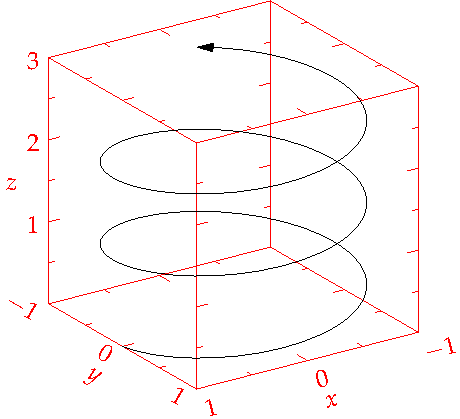
\includegraphics[width=\linewidth]{helix}
    \caption{Interacción entre dos cargas.}
    \label{fig:leycoulomb}
\end{marginfigure}

\textbf{La fuerza ejercida por una carga puntual sobre otra está dirigida a lo largo de la línea que las une. Es repulsiva si las cargas tienen el mismo signo y atractiva si tienen signos opuestos. La fuerza varía inversamente proporcional al cuadrado de la distancia que separa las cargas y es proporcional al valor de cada una de ellas.}

La fuerza ejercida por una carga puntual $q_1$ (en $r_1$) sobre otra carga puntual $q_2$ (en $r_2$) se define como:

\begin{equation}
    \vec{F}_{12} = K\displaystyle\frac{q_1q_2}{r_{12}^2}\hat{r}_{12}~[N],
\end{equation}

donde $K$ es la constante de Coulomb cuyo valor depende del medio en el que se produzca la interacción\sidenote{La constante dieléctrica $K = 1/r\pi\epsilon_0 = 9\cdot10^9~[N\cdot m^2 \cdot C^{-2}]$ siendo $\epsilon_0 = 8.85\cdot 10^{-12}~[C^2\cdot N^{-1}\cdot m^{-2}]$ la permitividad del vacío.  Si el medio es distinto al vacío, $K$ cambia dado que la permitividad del mismo $\epsilon$ cambia ($\epsilon_0 \neq \epsilon$) $K' = 1/4\pi\epsilon$.}, $r_{12}$ es el módulo del vector $\vec{r}_{12} = \vec{r}_2 - \vec{r}_1$ que apunta de $q_1$ a $q_2$, y $\hat{r}_{12} = \vec{r}_{12} / r_{12}$ es el vector unitario del mismo.

\paragraph{Sistema de cargas} en el caso de un sistema de cargas, cada una de ellas ejerce una fuerza sobre las demás. La fuerza neta de cada carga es la suma vectorial de las fuerzas individuales. Esta es una consecuencia del principio de superposición de las fuerzas.

\newpage

\subsection{Campo Eléctrico}

\textbf{La interacción entre cargas eléctricas no se produce de forma instantánea sino que el intermediario de la fuerza mutua es el campo eléctrico. Su unidad es el newton por culombio $[NC^{-1}]$. La forma de determinar si en una cierta región existe un campo eléctrico es colocar una carga de prueba positiva $q_0$ y comprobar la fuerza que experimenta}:

\begin{equation}
\vec{F}{q,q_0} = K\frac{q q_0}{r^2_{12}}\hat{r}_{12}~[N].
\end{equation}

Así pues, el campo eléctrico se define como la fuerza por unidad de carga positiva en un punto determinado:

\begin{equation}
\vec{E} = \frac{\vec{F}}{q_0} = K \frac{q}{r^2}{\vec{r}}~[N\cdot C^{-1}],
\end{equation}

cuya dirección y sentido coincide con el de la fuerza eléctrica. De hecho, la fuerza eléctrica ejercida por una carga testigo $q_0$ en cualquier punto está relacionada con el campo eléctrico en dicho punto de forma análoga $\vec{F} = q_0\vec{E}$.

De forma general, el campo $\vec{E}$ en un punto $p$ en $r_p$ debido a una carga puntual $q_i$ situada en $r_i$ es:

\begin{equation}
\vec{E}_{ip} = K \frac{q_i}{r^2_{ip}}\hat{r}_{ip}~[N\cdot C^{-1}]
\end{equation}

\paragraph{Sistema de Cargas} el campo eléctrico cumple el principio de superposición por lo que el campo eléctrico resultante en un punto $p$ debido a una distribución de cargas puntuales $q_i$ se determina sumando los campos originados por cada carga $\vec{E}_p = \sum_i \vec{E}_{ip}$.

\begin{marginfigure}%
    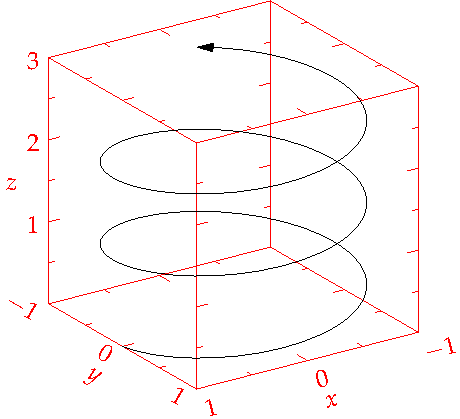
\includegraphics[width=\linewidth]{helix}
    \caption{Líneas de campo eléctrico para dos cargas iguales.}
    \label{fig:lineascampoelectrico}
\end{marginfigure}

\paragraph{Líneas de Campo Eléctrico} la forma de representar gráficamente un campo eléctrico es mediante las denominadas líneas de campo. Las líneas de campo eléctrico se dibujan de forma que el vector $\vec{E}$ sea tangente a ellas en cada punto. Su sentido coincide con el de dicho vector y deben cumplir la siguientes reglas:

\begin{itemize}
    \item Salen de cargas positivas y entran en negativas.
    \item Nunca se cortan.
    \item El número es proporcional al valor de la carga.
    \item Empiezan o terminan solo en cargas puntuales.
    \item La densidad es proporcional al valor del campo.
\end{itemize}

\subsection{Movimiento de Cargas Puntuales}

Cuando una carga eléctrica $q$ se coloca en el seno de un campo eléctrico $\vec{E}$, experimenta la acción de una fuerza eléctrica $\vec{F} = q\vec{E}$. Si la fuerza eléctrica es una única fuerza significativa que actúa sobre la partícula \sidenote{Si actúan varias fuerzas eléctricas se aplica el principio de superposición.}, podemos calcular la aceleración que experimenta dicha partícula mediante la Segunda Ley de Newton:

\begin{equation}
\vec{F} = m\vec{a} \rightarrow \vec{a} = \frac{\vec{F}}{m} = \frac{q\vec{E}}{m}~[m\cdot s^{-2}]~.
\end{equation}

\subsection{Dipolo Eléctrico}

\textbf{Un sistema de dos cargas iguales y opuestas $q$ separadas una distancia pequeña $L$ se denomina dipolo eléctrico.} Su intensidad y su orientación se definen mediante el momento dipolar eléctrico, un vector que apunta de la carga negativa a la positiva y cuyo valor es

\begin{marginfigure}%
    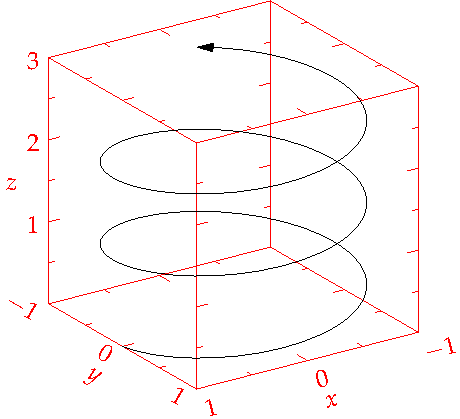
\includegraphics[width=\linewidth]{helix}
    \caption{Dipolo eléctrico.}
    \label{fig:dipolo}
\end{marginfigure}

\begin{equation}
\vec{p} = q\vec{L}~[C\cdot m],
\end{equation}

siendo $\vec{L}$ un vector cuyo origen está en la carga negativa y su extremo en la positiva. En la configuración de dipolo típica calculamos el campo eléctrico en cualquier punto de la mediatriz que une ambas cargas. En este caso, la distancia de cada carga a la mediatriz es $a$ y por lo tanto $\vec{p} = -2aq\hat{i}$ ya que el campo eléctrico sobre la mediatriz:

\begin{equation}
\vec{E} = K\frac{2aq}{(r^2 + a^2)^{3/2}}\hat{i} = K\frac{2aq}{r^3}\hat{i}~[N\cdot C^{-1}]~.
\end{equation}

Si aplicamos un campo eléctrico sobre un dipolo, no se ejerce una fuerza neta pero aparece un par de fuerzas que tiende a alinear el dipolo con el campo eléctrico, es decir, tiende a situar el momento dipolar $\vec{p}$ en la dirección del campo eléctrico $\vec{E}$. El momento del par de fuerzas es:

\begin{equation}
\vec{\tau} = \vec{L} \times q\vec{E} = q\vec{L} \times \vec{E} = \vec{p} \times \vec{E}~.
\end{equation}

Cuando el dipolo gira un ángulo $d\theta$, el campo eléctrico realiza un trabajo $dW = -\tau d\theta = -pE\sin{\theta}d\theta$. Igualando el trabajo con la variación de energía potencial $dU = -dW = pE\sin{\theta}d\theta$ e integrando $U = -pE\cos{\theta} + U_0$. Si tomamos como cero la energía potencial en $\theta = 90~[deg]$ entonces la energía potencial del dipolo es $U = -pE\cos{\theta} = -\vec{p}\cdot \vec{E}~[J]$.

\newpage

\subsection{Distribuciones Continuas de Carga}

A escala microscópica, la carga está cuantizada; sin embargo, en ocasiones se presentan situaciones en las que un gran número de cargas están tan próximas que la carga total puede considerarse distribuida en el espacio de forma continua. Para estas ocasiones se utiliza el concepto de densidad de carga continua. En este caso, se divide la distribución en pequeños elementos diferenciales de carga $dq$ de forma que el diferencial de campo eléctrico creado por cada una de ellas es

\begin{equation}
d\vec{E} = K\frac{dq}{r^2}\hat{r}~[N\cdot C^{-1}]~,
\end{equation}

así pues, el campo eléctrico total se calcula integrando

\begin{equation}
\vec{E} = \int K\frac{dq}{r^2}\hat{r}~[N\cdot C^{-1}]~.
\end{equation}

\paragraph{Distribución Lineal} en el caso de una distribución lineal, la densidad lineal de carga es $\lambda = dq / dl$ y su campo eléctrico en un punto dado se calcula integrando sobre la longitud $\vec{E} = \int_L K\lambda\frac{dl}{r^2}\hat{r}~[N\cdot C^{-1}]$.

\paragraph{Distribución Superficial} en el caso de una distribución superficial, la densidad superficial de carga es $\sigma = dq / ds$ y su campo eléctrico en un punto dado se calcula integrando sobre la superficie $\vec{E} = \int_S K\sigma\frac{ds}{r^2}\hat{r}~[N\cdot C^{-1}]$.

\paragraph{Distribución Volumétrica} en el caso de una distribución volumétrica, la densidad volumétrica de carga es $\rho = dq / dv$ y su campo eléctrico en un punto dado se calcula integrando sobre el volumen $\vec{E} = \int_V K\rho\frac{dv}{r^2}\hat{r}~[N\cdot C^{-1}]$.

\subsection{Flujo Eléctrico}

El flujo eléctrico es la magnitud matemática relacionada con el número de líneas de campo que atraviesa una superficie determinada. Las unidades del flujo son $[N\cdot m^2 \cdot C^{-1}]$ ya que, en su forma general el flujo se define como

\marginnote{Por lo general, la superficie suele ser perpendicular a $\vec{E}$ por lo que $\vec{E}\hat{n} = E$ y por lo tanto la expresión se simplifica simplemente a $\phi = EA$. En otros casos, la superficie forma un ángulo determinado $\theta$ y la expresión queda $\phi = EA\cos{\theta}$.}

\begin{equation}
\phi = \int_S \vec{E}d\vec{S} = \int_S \vec{E}\hat{n}dS~[N\cdot m^2 \cdot C^{-1}]~.
\end{equation}

Para una superficie cerrada el flujo será negativo si las líneas de campo entran y positivo si las líneas salen

\begin{equation}
\phi = \oint_S \vec{E}d\vec{S} = \oint_S \vec{E}\hat{n}dS~[N\cdot m^2 \cdot C^{-1}]~.
\end{equation}

\subsection{Ley de Gauss}

\begin{marginfigure}%
    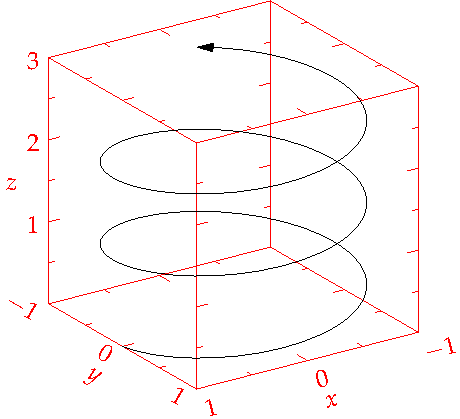
\includegraphics[width=\linewidth]{helix}
    \caption{Superficie esférica con carga $q$.}
    \label{fig:esferagauss}
\end{marginfigure}

La Ley de Gauss relaciona el flujo de campo eléctrico a través de una superficie cerrada y la carga encerrada en ella. Afirma que el flujo eléctrico neto a través de cualquier superficie cerrada es igual a la carga neta que se encuentre dentro de la misma dividida por la permitividad eléctrica:

\begin{equation}
\phi = \oint_S \vec{E}\hat{n}dS = 4\pi Kq = \frac{q}{\epsilon_0}~[N\cdot m^2 \cdot C^{-1}]~,
\end{equation}

todo ello con total independencia de la forma de la distribución, únicamente de la carga que se halle en su interior. Es válida para todas las superficies y distribuciones de carga.

\subsection{Diferencia de Potencial}

La fuerza ejercida por un campo eléctrico $\vec{E}$ sobre una carga puntual $q$ es $\vec{F} = q\vec{E}$. Cuando dicha carga experimenta un desplazamiento $d\vec{l}$, la variación de energía potencial electrostática es $dU = -q\vec{E}\cdot d\vec{l}$. Así pues, la variación de energía potencial por unidad de carga se denomina diferencia de potencial $dV$:

\marginnote{Es importante destacar que el potencial es una magnitud escalar, al contrario que el campo eléctrico que es una magnitud vectorial.}

\marginnote{Además, la función potencial es continua en todos los puntos excepto en aquellos en los que el campo eléctrico es infinito mientras que el campo eléctrico presenta discontinuidad en puntos donde existe carga superficial.}

\marginnote{La variación de energía potencial se relaciona también con el trabajo que cuesta desplazar una carga de forma que $W= -\Delta U$. Por lo que $\Delta V = -W_{ab}/q$.}

\marginnote{La variación de potencial se relaciona con el campo eléctrico ya que $dW = \vec{F}d\vec{r}$ por lo que $W = q\vec{E}\Delta\vec{r}$ y como $W = -q\Delta V$ entonces $\Delta V = -\vec{E}d\vec{r}$.}

\begin{equation}
dV = \frac{dU}{q} = -\vec{E}\cdot d\vec{l}~[V]~,
\end{equation}

de modo que, para un desplazamiento finito desde el punto $a$ al punto $b$, la variación de potencial es

\begin{equation}
\Delta V = V_b - V_a = \frac{\Delta U}{q} = -\int_a^b \vec{E}\cdot d\vec{l}~[V]~.
\end{equation}

\paragraph{Sobre el potencial y las líneas de campo:} las líneas de campo eléctrico señalan la dirección en la que el potencial eléctrico disminuye más rápidamente. Dado que $U = qV$, para una carga positiva, la región del espacio en la que existe menor energía potencial es también la de menor potencial eléctrico, motivo por el cual las cargas positivas se dirigen a las zonas con menor potencial eléctrico.

\subsection{Potencial Debido a Un Sistema de Cargas}

El potencial eléctrico en un punto $p$ a una distancia $r$ de una carga puntual $q$ puede calcularse a partir de la expresión $V_p - V_{ref} = -\int_{ref}^p \vec{E}\cdot d\vec{l}$. Teniendo en cuenta que el campo eléctrico debido a una carga puntual es $\vec{E} = kq/r^2 \hat{r}$, sutituyendo en la expresión anterior:

\begin{equation}
V_p - V_{ref} = -\int_{ref}^p \vec{E}\cdot d\vec{l} = -\int_{ref}^p \frac{kq}{r^2}\hat{r}\cdot d\vec{l} = -\int_{r_{ref}}^{r_p}\frac{kq}{r^2}dr~,
\end{equation}

poniendo $V_{ref} = 0$ e integrando a lo largo del camino desde un punto arbitrario de referencia:

\begin{equation}
V_p = -kq\int_{r_{ref}}^{r_p}\frac{1}{r^2}dr = \frac{kq}{r_p} - \frac{kq}{r_{ref}}~,
\end{equation}

dado que el punto de referencia es arbitrario, podemos elegir aquél que simplifique la ecuación y por lo tanto tomaremos el más lejano a la carga puntual $r_{ref} \rightarrow \infty$ y por lo tanto

\begin{equation}
V = \frac{kq}{r}~[V]~.
\end{equation}

El potencial en un punto debido a diversas cargas puntuales es igual a la suma de los potenciales debidos a cada carga por separado (principio de superposición):

\begin{equation}
V = \sum_i \frac{kq_i}{r_i}~[V]~.
\end{equation}

\subsection{Relación General entre $\vec{E}$ y V}

Las componentes cartesianas del campo eléctrico están relacionadas con las derivadas parciales del potencial respecto a $x$, $y$ o $z$ de la siguiente manera:

\begin{equation}
\vec{E} = -\vec{\nabla}V = -(\frac{\partial V}{\partial x}\hat{i} + \frac{\partial V}{\partial y}\hat{j} + \frac{\partial V}{\partial z}\hat{k})
\end{equation}

\subsection{Potencial en Distribuciones Continuas de Carga}

El potencial debido a una distribución continua de carga puede calcularse eligiendo un elemento de carga $dq$ que puede considerarse como una carga puntual y tomando en consideración el principio de superposición e integrando tal y como hicimos con el campo eléctrico: \sidenote{Esta expresión supone que $V_\infty = 0$ y por ello no puede utilizarse cuando la carga se encuentra en el infinito, como es el caso de las distribuciones infinitas de carga.}

\begin{equation}
V = \int dV = \int \frac{k dq}{r}~[V]
\end{equation}

\subsection{Superficies Equipotenciales}

Es el lugar geométrico de todos los puntos que se encuentran al mismo potencial. Cumplen la condición de encontrarse en un plano perpendicular al campo eléctrico. El trabajo para mover una partícula entre dos puntos a lo largo de una superficie equipotencial es nulo ya que $W_{ab} = -q\Delta V$ y $\Delta V = 0$.

\subsection{Energía Potencial Electrostática}

La energía potencial electrostática de un sistema de cargas puntuales es el trabajo necesario para llevar las cargas desde el infinito a sus posiciones finales:

\begin{equation}
U = \frac{1}{2}\sum_i q_iV_i ~[J]
\end{equation}

\subsection{Conductores}

\textbf{Un conductor es un material que se caracteriza por tener cargas libres que pueden moverse en su interior.}

Si sometemos un conductor a un campo eléctrico externo, su carga libre se redistribuye hasta anular el campo eléctrico en su interior. En estas condiciones se dice que el conductor está en equilibrio electrostático. El campo eléctrico $E'$ generado por las cargas redistribuidas anula al campo eléctrico externo $E_0$ ($E' = E_0$).

\paragraph{Toda carga libre en un conductor se coloca en su superficie. } Suponiendo una superficie gaussiana justo en el interior de la superficie del conductor, como el campo eléctrico es nulo, también lo será en todos los puntos de la superficie gaussiana y por lo tanto, el flujo eléctrico también es nulo. Esto significa que la carga encerrada es nula y por lo tanto, de existir carga, debe estar en su superficie.

\paragraph{El campo eléctrico en la superficie del conductor es perpendicular a dicha superficie y vale $\sigma / \epsilon_0$.} Tomamos como superficie gaussiana un cilindro con una cara en el exterior y otra en el interior del conductor. Si el conductor está en equilibrio, el campo eléctrico en la superficie debe ser perpendicular a la misma por lo que solo hay flujo a través de la cara superior del cilindro $\phi = ES = q / \epsilon_0$, $q = \sigma S$ por lo que $E = \sigma / \epsilon_0$.

\subsection{Condensadores}

\textbf{Un condensador es un dispositivo constituido por dos placas conductoras paralelas rellenas normalmente con un material dieléctrico no conductor.}

La magnitud que caracteriza a un condensador es su capacidad, su unidad es el Faradio $[F] = [C/V]$. La capacidad se define como: \sidenote{En el caso de un condensador esférico $C = Q/V = Q/kQ/R = R/k = 4\pi\epsilon_0 R~[F]$.}

\begin{equation}
C = \frac{Q}{V}~[F]~,
\end{equation}

siendo $Q$ la carga almacenada en cada placa y $V$ la diferencia de potencial entre las mismas.

\paragraph{Condensador de Placas Paralelas} en este caso, cada placa tiene un área $A$ y están separadas una distancia $d$. Situando una carga $+Q$ en una placa y una carga $-Q$ en la otra, cada placa contribuye con un campo eléctrico $E = \sigma/2\epsilon_0$, resultando así un campo total $E = \sigma /\epsilon_0$. Como el campo que existe entre las placas es uniforme, su diferencia de potencial es igual a $V = Ed$.

\begin{equation}
V = Ed = \frac{\sigma}{\epsilon_0}d = \frac{Qd}{\epsilon_0A}~[V]~,
\end{equation}

y por lo tanto su capacidad es

\begin{equation}
C = \frac{Q}{V} = \frac{Q}{Qd/\epsilon_0A} = \frac{\epsilon_0A}{d}~[F]~.
\end{equation}

\marginnote{Como $V$ es proporcional a $Q$, la capidad no depende ni de uno ni de otro. La capacidad depende de la geometría (del área de las placas y de la distancia de separación en el caso del condensador de placas paralelas).}

\paragraph{Condensador de Placas Cilíndricas} en un condensador cilíndrico formado por dos conductores de longitud $L$, uno de ellos con radio $R_1$ y el otro de radio $R_2$, podemos obtener su capacidad $C = Q/V$ calculando en primer lugar el campo eléctrico utilizando la Ley de Gauss y posteriormente integrándolo entre $R_1$ y $R_2$ para obtener la diferencia de potencial $V = |V_{R_2} - V_{R_1}|$.

\begin{equation}
C = \frac{Q}{V} = \frac{2\pi\epsilon_0L}{\ln{R_2/R_1}}~[F]~.
\end{equation}

\subsection{Almacenamiento de la Energía Eléctrica}

Inicialmente, el condensador se compone de dos conductores descargados. Durante el proceso de carga se transfiere una cierta carga $q$ por lo que su diferencia de potencial es $V = q/C$. Si se transfiere ahora una pequeña cantidad de carga $dq$ desde el conductor negativo (con potencial $V=0$) hacia el conductor positivo (con un potencial $V$), la energía potencial del condensador se incrementa

\begin{equation}
dU = V dq = \frac{q}{C}dq~[J]~,
\end{equation}

dicha energía potencial va aumentando por lo que su valor final se alcanza cuando la carta total es $Q$ y lo podemos calcular como la integral de los incrementos de energía

\begin{equation}
U = \int dU = \int_0^Q \frac{q}{C}dq = \frac{1}{C}\int_0^Q qdq = \frac{1}{2}\frac{Q^2}{C}~[J]~.
\end{equation}

Esta energía potencial es la energía almacenada en el condensador y dado que $C = Q/V$, podemos expresar esta energía de varios modos:

\begin{equation}
U = \frac{1}{2}\frac{Q^2}{C} = \frac{1}{2}QV = \frac{1}{2}CV^2~[J]~.
\end{equation}

Por otro lado, es posible relacionar la energía almacenada en el condensador con el campo eléctrico existente para obtener la energía del campo electrostático. Dado que la diferencia de potencial $V = Ed$ y la capacidad viene dada por $C = \epsilon_0 A/d$, la energía almacenada es

\begin{equation}
U = \frac{1}{2}CV^2 = \frac{1}{2}\frac{\epsilon_0A}{d}(Ed)^2 = \frac{1}{2}\epsilon_0E^2(Ad)~[J]~,
\end{equation}

como el producto $Ad$ es el volumen del espacio comprendido entre las placas, podemos determinar la energía por unidad de volumen (la densidad de energía $u_e$) como:

\begin{equation}
u_e = \frac{1}{2}\epsilon_0E^2~[J\cdot m^{-3}]~.
\end{equation}

\subsection{Dieléctricos}

Un material no conductor se denomina dieléctrico. Cuando el espacio entre los conductores de un condensador se ve ocupado por un dieléctrico, la capacidad aumenta en un factor $k$ característico del dieléctrico (ya que el campo se debilita a causa de dicho material). Así pues, la diferencia de potencial se reduce y por lo tanto la relación $Q/V$ aumenta. 

\begin{equation}
E = \frac{E_0}{k}
\end{equation}

\begin{equation}
C = kC_0
\end{equation}

Siendo $k$ la constante dieléctrica $\epsilon = k\epsilon_0$.

\subsection{Asociación de Condensadores}

En serie, las caídas de voltaje se suman por lo que:

\begin{equation}
\frac{1}{C_{eq}} = \sum_i \frac{1}{C_i}~[F]
\end{equation}

En paralelo, el voltaje en sus extremos es el mismo:

\begin{equation}
C_{eq} = \sum_i C_i~[F]
\end{equation}

\clearpage

\section{Corriente Continua}

\clearpage

\section{Campo Magnético}

\clearpage

\section{Inducción Magnética}

\subsection{Flujo Magnético}

\begin{marginfigure}%
    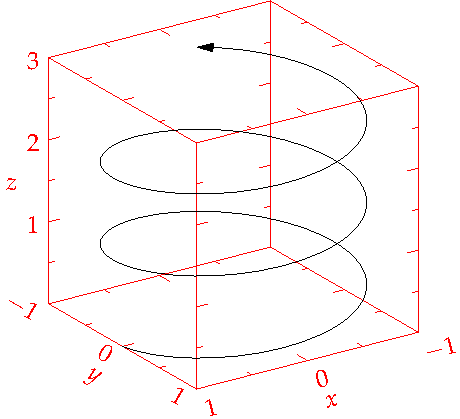
\includegraphics[width=\linewidth]{helix}
    \caption{Superficie, campo y flujo magnético.}
    \label{fig:flujomagnetico}
\end{marginfigure}

El flujo magnético $\phi_m$ a través de una superficie $A$ se calcula de forma análoga al flujo de un campo eléctrico. Siendo $dA$ un elemento de área infinitesimal de dicha superficie y $\hat{n}$ el vector unitario perpendicular a dicho elemento \sidenote{Podemos observar además que, si bien hay dos direcciones normales posibles, su elección es arbitraria y el signo del flujo no depende de dicha elección.}, el flujo queda definido como sigue (siendo su unidad el \emph{Weber} $[Wb]$ que equivale a $[T\cdot m^2]$)

\begin{equation}
\phi_m = \int_{S} \mathbf{\vec{B}}\mathbf{\hat{n}}dA = \int_{S}B_ndA ~ [Wb]~, 
\end{equation}

Dado que el campo magnético es proporcional al número de líneas de campo por unidad de área, el flujo es proporcional al número de líneas que atraviesan dicha superficie. Por lo tanto, si la superficie es un plano de área $A$ y el campo magnético es constante sobre la superficie, el flujo que la atraviesa es

\begin{equation}
\phi_m = \mathbf{\vec{B}}\mathbf{\hat{n}}A = BA\cos{\theta} ~ [Wb]~,
\end{equation}

donde $\theta$ es el ángulo que forman el campo magnético y la normal de la superficie. Frecuentemente, esta aproximación se utiliza para calcular el flujo magnético a través de una superficie rodeada por una bobina con $N$ espiras

\begin{equation}
\phi_m = N\mathbf{\vec{B}}\mathbf{\hat{n}}A = NBA\cos{\theta} ~ [Wb]~.
\end{equation}

\begin{marginfigure}%
    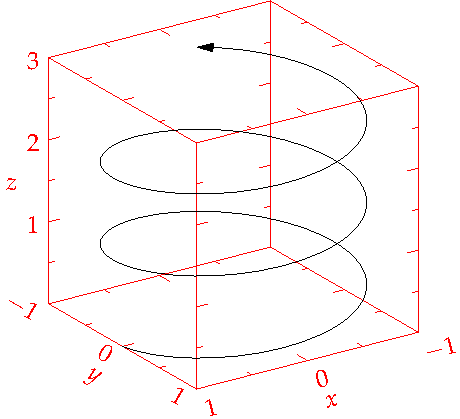
\includegraphics[width=\linewidth]{helix}
    \caption{Flujo magnético a través de una superficie $S$ encerrada por una bobina con $N$ espiras o vueltas.}
    \label{fig:flujomagneticoespira}
\end{marginfigure}

\subsection{FEM Inducida y Ley de Faraday}

Si el flujo magnético a través de un área rodeada por un circuito varía por cualquier motivo, se induce una FEM que es igual en módulo a la variación por unidad de tiempo del flujo que atraviesa dicho circuito:

\begin{equation}
\mathcal{E} = -\displaystyle\frac{d\phi_m}{dt}~[V]~.
\end{equation}

Los campos eléctricos estudiados con anterioridad eran producidos por cargas eléctricas estáticas por lo que su circulación (potencial como $\oint_{C}\mathbf{\vec{E}}\cdot d\mathbf{\vec{l}}$) alrededor de una curva cerrada $C$ era cero. No obstante, el campo eléctrico generador por un campo magnético variable no es conservativo ya que su circulación (potencial) es una FEM inducida por el flujo magnético que atraviesa cualquier superficie $S$ encerrada por $C$ tal y como comentamos anteriormente

\begin{equation}
\mathcal{E} = \oint_{C}\mathbf{\vec{E}_{nc}}\cdot d \mathbf{\vec{l}} = -\displaystyle\frac{d}{dt}\int_{S}\mathbf{\vec{B}}\cdot\mathbf{\hat{n}}dA = -\displaystyle\frac{d\phi_m}{dt}~[V]~.
\end{equation}

\subsection{Ley de Lenz}

\begin{marginfigure}%
    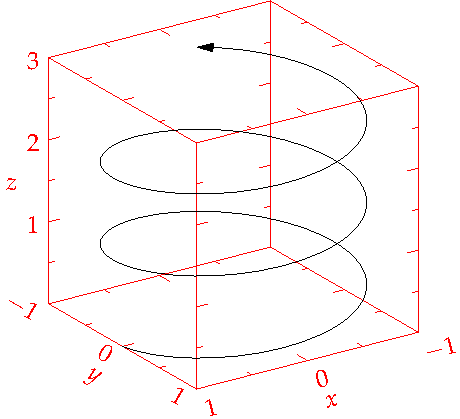
\includegraphics[width=\linewidth]{helix}
    \caption{Ejemplo de la Ley de Lenz.}
    \label{fig:ejemplolenz}
\end{marginfigure}

Cuando se produce una variación del flujo magnético que atraviesa una superficie, el campo magnético debido a la corriente inducida genera un flujo magnético sobre la misma superficie que se opone a dicha variación. Dicho de otro modo, la Ley de Lenz es la responsable del signo negativo en la Ley de Faraday puesto que la FEM y la corriente inducidas poseen una dirección y sentido tal que tienden a oponerse a la variación que las produce.

\subsection{FEM de Movimiento}

La FEM inducida en un conductor que se mueve a través de un campo magnético se denomina FEM de movimiento. El ejemplo más claro es el de una varilla conductora que se desliza a lo largo de dos conductores unidos a una resistencia, todo ello en el seno de un campo magnético uniforme tal y como se muestra en la Figura \ref{fig:femmovimiento}.

\begin{marginfigure}%
    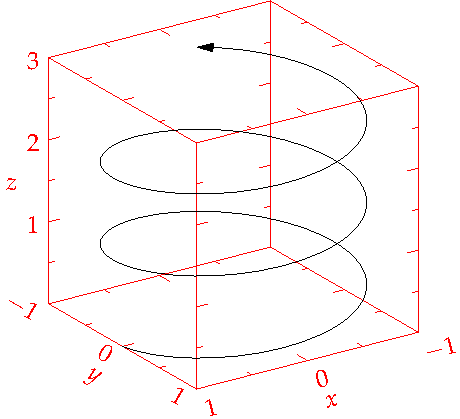
\includegraphics[width=\linewidth]{helix}
    \caption{Varilla conductora deslizante sobre raíles conductores (conectados a una resistencia) en el seno de un campo magnético.}
    \label{fig:femmovimiento}
\end{marginfigure}

En este caso, el área de la superficie $S$ encerrada por el circuito se incrementa cuando la varilla se desplaza a la derecha por lo que el flujo magnético a través de la misma también crece y por ello se induce una FEM en el circuito. Si denominamos $l$ a la distancia entre los raíles y $x$ a la distancia entre el extremo izquierdo de los raíles y la varilla, el área es $lx$ y por lo tanto el flujo es

\begin{equation}
\phi_m = BA = Blx~[Wb].
\end{equation}

Si derivamos respecto al tiempo para obtener la variación del flujo respecto al mismo (teniendo en cuenta que $x$ varía con el tiempo \sidenote{La variación de la longitud $x$ con el tiempo es simplemente la velocidad a la que se desplaza la varilla $v = \displaystyle\frac{dx}{dt}$})

\begin{equation}
\displaystyle\frac{d\phi_m}{dt} = Bl\displaystyle\frac{dx}{dt} = Blv~[V]~,
\end{equation}

podemos deducir que la FEM inducida en el circuito es

\begin{equation}
\mathcal{E} = -\displaystyle\frac{d\phi_m}{dt} = -Blv~[V]
\end{equation}

\subsection{Generadores y Motores}

Un generador de corriente alterna se puede construir mediante una bobina giratoria en el seno de un campo magnético uniforme. Los extremos de la bobina se conectan a un anillo deslizante que gira con la bobina. Cuando la bobina gira por acción mecánica, el flujo magnético a través de ella varía y por lo tanto se induce una FEM en ella. El ángulo formado entre el campo magnético $\mathbf{\vec{B}}$ y la normal de la superficie de la bobina $\mathbf{\hat{n}}$ viene dado por

\begin{marginfigure}%
    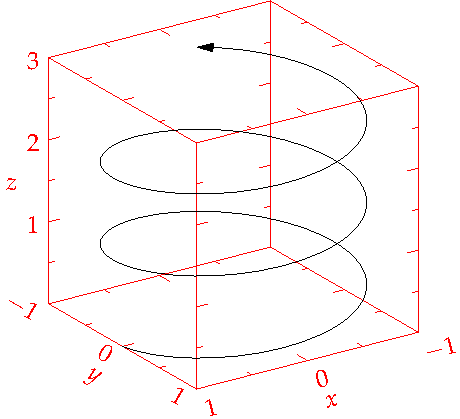
\includegraphics[width=\linewidth]{helix}
    \caption{Generador de corriente alterna en el que una bobina girando con velocidad angular constante en el seno de un campo magnético genera una FEM inducida sinusoidal.}
    \label{fig:generadorac}
\end{marginfigure}

\begin{equation}
\theta = \omega t~[deg]~,
\end{equation}

por lo tanto, el flujo magnético que atraviesa la bobina depende del tiempo y de la velocidad angular de rotación de la misma como sigue

\begin{equation}
\phi_m = NBA\cos{\omega t} = NBA\cos{2\pi f}~[Wb]~.
\end{equation}

Podemos deducir entonces que la FEM producida por la bobina es 

\begin{equation}
\mathcal{E} = - \displaystyle\frac{d\phi_m}{dt} = \omega NBA\sin{\omega t} = \mathcal{E}_{max} \sin{\omega t} ~[V]~,
\end{equation}

donde

\begin{equation}
\mathcal{E}_{max} = \omega NBA~[V]~.
\end{equation}

\subsection{Inductancia}

El flujo magnético generado a través de una bobina por una corriente que circula por la misma es proporcional a la intensidad de corriente según una constante $L~[H]$ \sidenote{La unidad del sistema internacional para la inductancia $L$ es el Henry $[H]$.}

\begin{equation}
\phi_m = LI~[Wb]~,
\end{equation}

esta constante se denomina autoinducción y depende de la geometría de la bobina. Para el caso de un solenoide enrollado determinamos anteriormente que el flujo máximo venía dado por $NBA$, por lo que desarrollando esta igualdad

\begin{equation}
\phi_m = NBA = N(\mu_0 nI)A = \mu_0 n^2 IAl~[H]~,
\end{equation}

ya que el campo magnético es conocido $B=\mu_0 nI$ y el número de vueltas de la bobina también $N=nl$. La constante de proporcionalidad respecto a la intensidad de corriente es la autoinducción y únicamente depende de factores geométricos

\begin{equation}
L = \phi_m / I = \mu_0 n^2 Al~[H]~.
\end{equation}

\subsection{Energía Magnética}

De la misma forma que un condensador almacena energía eléctrica, un inductor almacena energía magnética. La energía almacenada en un inductor que transporta una corriente $I$ es

\begin{equation}
U_m = \displaystyle\frac{1}{2}LI^2~[J]~.
\end{equation}

Esa energía magnética puede ser expresada como

\begin{equation}
U_m = \displaystyle\frac{1}{2}LI^2 = \displaystyle\frac{1}{2}\mu_0n^2Al(\displaystyle\frac{B}{\mu_0 n})^2 = \displaystyle\frac{B}{\mu_0 n}^2Al~[J]~,
\end{equation}

y a partir de la misma podemos derivar la densidad de energía magnética $u_m$ como la energía por unidad de volumen $Al$

\begin{equation}
u_m = \displaystyle\frac{B^2}{2\mu_0}~[J\cdot m^{-3}]~.
\end{equation}

\subsection{Circuitos RL}

\begin{marginfigure}%
    \centering
    \begin{circuitikz}
\draw (0,0)
  to[V=$V_{in}$, invert] (0,2) % The voltage source
  to[R=\(R_1\)] (3,2) % The resistor
  to[L=\(L_1\)] (3,0) % The inductor
  to (0,0); %Inductor One
\end{circuitikz}
    \bigskip
    \caption{Circuito RL básico.}
    \label{fig:circuitorl}
\end{marginfigure}

Un circuito RL (ver Figura \ref{fig:circuitorl}) es todo aquel que contiene una resistencia y un inductor. La aplicación de la regla de las mallas de Kirchoff arroja la siguiente expresión para el circuito

\begin{equation}
\mathcal{E}_0 - IR - L\displaystyle\frac{dI}{dt} = 0
\end{equation}

En el instante inicial, la corriente es nula por lo que $IR$ es cero y la FEM de la batería es igual a la caída de potencial en el inductor. Cuando la corriente comienza a crecer, $IR$ crece y la variación de la corriente con el tiempo disminuye \sidenote{Cuando la inductancia $L$ no es despreciable, $I$ no puede saltar súbitamente de cero a un valor finito sino que $dI/dt$ es finita y por lo tanto la corriente es continua en el tiempo.} hasta que en un tiempo breve, la corriente alcanza un valor positivo $I$. Su variación con el tiempo podemos resolverla separando variables e integrando

\begin{equation}
\displaystyle\frac{dI}{dt} = \mathcal{E} - \displaystyle\frac{IR}{L} \rightarrow \displaystyle\frac{dI}{\mathcal{E}-IR} = \displaystyle\frac{dt}{L}
\end{equation}

\marginnote{Cuanto mayor es la autoinducción $L$ o menor es la resistencia $R$ del circuito, más tiempo es necesario para establecer una fracción determinada de la corriente final $I_0$.}

\begin{equation}
I(t) = \displaystyle\frac{\mathcal{E}}{R}(1 - e^{-\displaystyle\frac{R}{L}t}) = I_0 (1 - e^{-\displaystyle\frac{t}{\tau}})~[A]~,
\end{equation}

donde $I_0$ es el valor máximo o final de la corriente $\mathcal{E/R}~[A]$ cuando $t\rightarrow \infty$ y $\tau$ es la constante de tiempo o tiempo característico del circuito $L/R~[s]$.

\begin{figure*}[h]
    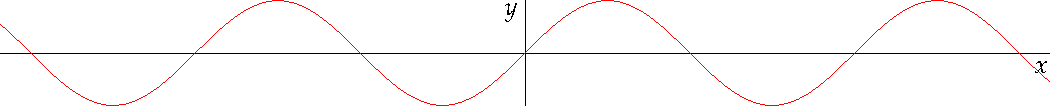
\includegraphics[width=\linewidth]{sine.pdf}%
    \caption{Variación de la intensidad de corriente en función del tiempo en un circuito RL.}%
    \label{fig:fullfig}%
  \end{figure*}


\clearpage

\section{Ondas Electromagnéticas}

\subsection{Corriente de Desplazamiento}

La Ley de Ampère relaciona la componente tangencial del campo magnético (integral lineal) alrededor de una curva cerrada $C$ con la corriente $I_S$ que atraviesa cualquier área $S$ limitada por dicha curva

\begin{equation}
\oint_C \mathbf{\vec{B}}\cdot d\mathbf{\vec{l}} = \mu_0 I_S~.
\end{equation}


\begin{marginfigure}%
    \centering
    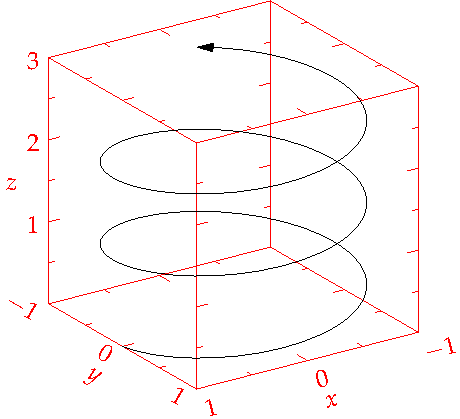
\includegraphics[width=\linewidth]{helix}
    \caption{Dos superficies $S_1$ y $S_2$ limitadas por la misma curva $C$. La corriente atraviesa la superficie $S_1$ pero no $S_2$. La ley de Ampère no es válida.}
    \label{fig:amperecondensador}
\end{marginfigure}

Sin embargo, esta afirmación no es siempre cierta: no es válida cuando la corriente no es continua, como por ejemplo sucede al interrumpirse en la placa de un condensador (ver Figura \ref{fig:amperecondensador}).

No obstante, Maxwell demostró que esta Ley sí puede generalizarse a todas las situaciones si sustituimos la corriente $I_S$ de la ecuación por la suma de dicha corriente $I_S$ y otro término $I_D$ conocido como corriente de desplazamiento de Maxwell y definido como

\begin{equation}
I_D = \mathcal{E}_0\displaystyle\frac{d\phi_E}{dt}~,
\end{equation}

siendo $\phi_e$ el flujo del campo eléctrico a través de la superficie limitada por la curva $C$ \sidenote{$\phi_e = \oint_S \mathbf{\vec{E}}\cdot d\mathbf{\vec{S}}$}. Así pues, la forma modificada de la Ley de Ampère, conocida como Ley de Ampère-Maxwell es

\begin{equation}
\oint_C \mathbf{\vec{B}}\cdot d\mathbf{\vec{l}} = \mu_0 (I_S + I_D) = \mu_0 I_S + \mu_0 \mathcal{E}_0\displaystyle\frac{d\phi_E}{dt}~.
\end{equation}

\subsection{Ecuaciones de Maxwell}

Maxwell dedujo que las leyes fundamentales de la electricidad y el magnetismo podían resumirse de form matemática en lo que se conocen como las Leyes de Maxwell. Estas ecuaciones relacionan los campos eléctricos y magnéticos con sus fuentes: cargas en reposo, corrientes y campos variables.

La primera de estas ecuaciones la Ley de Gauss para el campo eléctrico, la cual afirma que el flujo a través de una superficie cerrada es proporcional a la carga encerrada por la misma.

\begin{equation}
\oint_S \mathbf{\vec{E}}\cdot d\mathbf{\vec{S}} = \displaystyle\frac{Q_{int}}{\mathcal{E}_0}~[V\cdot m].
\end{equation}

La segunda ecuación es la Ley de Gauss del magnetismo, la cual implica la no existencia de monopolos magnéticos ya que en una superficie cerrada el número de líneas de campo que entran es igual a las que salen (el flujo es cero).

\begin{equation}
\oint_S \mathbf{\vec{B}}\cdot d\mathbf{\vec{S}} = 0~[Wb]~.
\end{equation}

La tercera ecuación es la Ley de Faraday, relacionando el flujo del campo magnético (a través de una superficie no cerrada) con el campo eléctrico.

\begin{equation}
\oint_C \mathbf{\vec{E}}\cdot d\mathbf{\vec{l}} = -\displaystyle\frac{d\phi_m}{dt} = -\displaystyle\frac{d}{dt}\int\mathbf{\vec{B}}\cdot d\mathbf{\vec{S}}~[V]~.
\end{equation}

La cuarta ecuación es la Ley de Ampère-Maxwell que expresa que la circulación de campo eléctrico es proporcional a la corriente y a la variación de flujo eléctrico.

\begin{equation}
\oint_C \mathbf{\vec{B}}\cdot d\mathbf{\vec{l}} = \mu_0 I_s + \mu_0 I_d = \mu_0 I_s + \mu_0 \epsilon_0 \displaystyle\frac{d}{dt}\oint_S \mathbf{\vec{E}}\cdot d\mathbf{\vec{S}}~.
\end{equation}

\subsection{Ecuación de Ondas Unidimensionales}

Las ondas obedecen a una ecuación de derivadas parciales denominada ecuación de onda

\begin{equation}
v^2 \displaystyle\frac{\partial^2 y(x,t)}{\partial x^2} = \displaystyle\frac{\partial^2 y(x,t)}{\partial t^2}~,
\end{equation}

donde $y(x,t)$ es la función de onda y $v$ es la velocidad de la misma \sidenote{En el caso de las ondas electromagnéticas que nos ocupan, la velocidad de onda es $c = 1/\sqrt{\mu_0 \epsilon_0}$}. Esta ecuación tiene una solución general en

\begin{equation}
y(x,t) = y_1(x - vt) + y_2(x + vt)~,
\end{equation}

donde $y_1$ e $y_2$ son funciones de $x-vt$ y $x+vt$ respectivamente y pueden expresarse como una superposición de funciones de onda armónicas

\begin{equation}
y_1(x,t) = y_0 \sin{(k(x - \omega t) + \phi)}
\end{equation}
\begin{equation}
y_2(x,t) = y_0 \sin{(k(x + \omega t) + \phi)}
\end{equation}

donde $y_0$ es la amplitud, $k = 2\pi / \lambda$ es el número de ondas, $\omega = 2\pi f$ es la frecuencia angular o velocidad de la onda y $\phi$ es la fase. Adicionalmente, $T = 2\pi/\omega~[s]$ es el período y se cumple la igualdad $\lambda v = c ~ [m\cdot s^{-1}]$. Además, $v = \lambda f$.

\subsection{Ondas Electromagnéticas}

Las ondas electromagnéticas planas son una solución de las ecuaciones de Maxwell en forma de ondas transversales con los campos $\mathbf{\vec{E}}$ y $\mathbf{\vec{B}}$ perpendiculares entre sí y a la dirección de propagación. Tanto $\mathbf{\vec{E}}$ como $\mathbf{\vec{B}}$ obedecen a ecuaciones de onda semejantes a las expuestas anteriormente. Si suponemos que $\mathbf{\vec{E}}$ y $\mathbf{\vec{B}}$ son funciones del tiempo y de una sola coordenada espacial que tomaremos como $x$, nos encontramos ante una onda plana que se propaga paralelamente al eje $x$ siendo las componentes $x$ de los campos nulas, de modo que $\mathbf{\vec{E}}$ y $\mathbf{\vec{B}}$ son perpendiculares al eje $x$ y obedecen a las siguientes ecuaciones de onda

\begin{equation}
c^2 \displaystyle\frac{\partial^2 \mathbf{\vec{E}}}{\partial x^2} = \displaystyle\frac{\partial^2 \mathbf{\vec{E}}}{\partial t^2}
\end{equation}

\begin{equation}
c^2 \displaystyle\frac{\partial^2 \mathbf{\vec{B}}}{\partial x^2} = \displaystyle\frac{\partial^2 \mathbf{\vec{B}}}{\partial t^2}
\end{equation}

\paragraph{Energía, Intensidad y Potencia}

Como todo tipo de onda, las ondas electromagnéticas transportan energía y momento. La energía viene descrita por la intensidad, es decir, la potencia media por unidad de área incidente sobre una superficie perpendicular a la dirección de propagación.

Si consideramos una onda propagándose en una región del espacio de forma cilíndrica con longitud $L$ y sección $A$, la energía electromagnética media $U_m$ dentro de esta región es igual a $u_m LA$ donde $u_m$ es la densidad de energía media y $LA$ es el volumen de la región cilíndrica. En el tiempo $\Delta t$ que emplea la onda en recorrer la longitud $L$, toda la energía pasa a través de una de las bases de la región cilíndrica. Dado que el tiempo $\Delta t$ es $L/c$, la potencia $P_m$ (energía por unidad de tiempo) que pasa por dicha base es

\begin{equation}
P_m = \displaystyle\frac{U_m}{\Delta t} = \displaystyle\frac{u_m LA}{L/c} = u_m Ac~,
\end{equation}

y por lo tanto, la intensidad (potencia media por unidad de área)

\begin{equation}
I = \displaystyle\frac{P_m}{A} = u_m c~.
\end{equation}

La densidad de energía de la onda $u$ es la suma de las densidades de energía eléctrica y magnética \sidenote{Cabe destacar que estas expresiones obedecen a una onda que se propaga en el vacío, de tratarse de otro medio las constantes $\epsilon_0$ y $\mu_0$ cambiarían.}

\begin{equation}
u_e = \displaystyle\frac{1}{2}\epsilon_0 E^2
\end{equation}

\begin{equation}
u_{mag} = \displaystyle\frac{1}{2}\displaystyle\frac{B^2}{\mu_0}
\end{equation}

En una onda electromagnética en el vacío, $E = cB$ por lo que podemos expresar la densidad de energía magnética en función del campo eléctrico y viceversa

\begin{equation}
u_{mag} = \displaystyle\frac{B^2}{2\mu_0} = \displaystyle\frac{(E/c)^2}{2\mu_0} = \displaystyle\frac{E^2}{2\mu_0c^2} = \displaystyle\frac{1}{2}\epsilon_0 E^2
\end{equation}

para finalmente determinar la densidad de energía total de la onda

\begin{equation}
u = u_e + u_{mag} = \displaystyle\frac{1}{2}\epsilon_0 E^2 + \displaystyle\frac{1}{2}\displaystyle\frac{B^2}{\mu_0} = \epsilon_0E^2
\end{equation}

\paragraph{Vector de Poynting}

El vector de Poynting $\mathbf{\vec{S}}$ apunta en la dirección de propagación de la onda electromagnética. El módulo medio del vector es la intensidad de la onda y su dirección es la dirección de propagación de la misma.

\begin{equation}
\mathbf{\vec{S}} = \displaystyle\frac{\mathbf{\vec{E}} \times \mathbf{\vec{B}}}{\mu_0}
\end{equation}

La intensidad (potencia por área) es el promedio temporal del módulo del vector de Poynting

\begin{equation}
I_{media} = \displaystyle\frac{1}{2}\displaystyle\frac{E_0B_0}{\mu_0} = \displaystyle\frac{1}{2}S_0
\end{equation}

\paragraph{Dirección de Propagación}

\begin{marginfigure}%
    \centering
    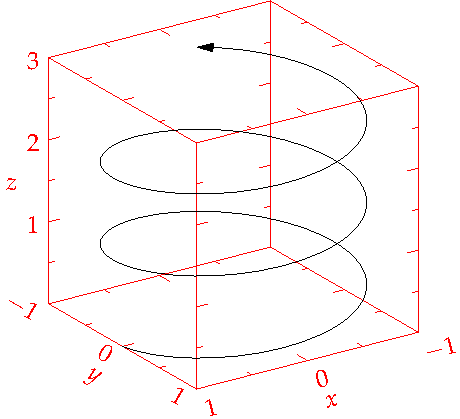
\includegraphics[width=\linewidth]{helix}
    \caption{Los vectores de campo eléctrico y campo magnético en una onda electromagnética. Los campos están en fase, perpendiculares entre sí y perpendiculares a la dirección de propagación de la onda.}
    \label{fig:ondaelectromagnetica}
\end{marginfigure}

Las ondas electromagnéticas son ondas transversales y los campos eléctrico y magnético están en fase y sus módulos relacionados, en cada punto del espacio, por la expresión $E = cB$ \sidenote{En el vacío.} donde $c$ es la velocidad de la onda. La dirección de propagación de una onda electromagnética es la dirección del producto vectorial $\mathbf{\vec{E}}\times\mathbf{\vec{B}}$. El vector de Poynting por lo tanto, apunta en la dirección de propagación de la onda electromagnética.

\paragraph{Momento y Presión}

El módulo del momento transportado por una onda electromagnética es

\begin{equation}
p = \displaystyle\frac{U_m}{c}~,
\end{equation}

como la potencia ($P_m$) de una onda es la energía por unidad de tiempo y la intensidad ($I$) es dicha potencia por unidad de área, la intensidad dividida por $c$ es el momento transportado por la onda por unidad de tiempo y área. El momento por unidad de tiempo es una fuerza, por lo tanto la intensidad de la onda dividida por $c$ es una fuerza por unidad de área que recibe el nombre de presión de radiación $P_r$

\marginnote{Considerando una onda electromagnética que incide sobre una superficie, si la superficie absorbe una energía $U$ de la onda electromagnética, también absorbe el momento $p$ y la presión ejercida sobre la misma es igual a la presión de radiación. Si la onda se refleja, el momento transferido es $2p$ ya que la onda transporta el momento en sentido opuesto.}

\begin{equation}
P_r = \displaystyle\frac{I}{c} = \displaystyle\frac{1}{2}\displaystyle\frac{E_0B_0}{\mu_0 c}~.
\end{equation}

\clearpage

\section{Óptica}

\subsection{Propagación de la Luz}

La propagación de la luz es gobernada por la ecuación de onda, aunque mucho antes de que Maxwell desarrollara su teoría de las ondas electromagnéticas, la propagación de la luz fue descrita empíricamente por dos principios atribuidos a Christian Hyugens y a Pierrre de Fermat.

\paragraph{Principio de Hyugens}

Cada punto de un frente de onda primario sirve como foco de ondas esféricas secundarias que avanzan con una velocidad y frecuencia igual a las de la onda primaria. El frente de onda primario al cabo de un cierto tiempo es envolvente de estas ondas elementales.

\paragraph{Principio de Fermat}

La trayectoria seguida por la luz para pasar de un punto a otro es aquella para la cual el tiempo de recorrido es un mínimo. O lo que es lo mismo, la luz tiende a recorrer el camino óptico por el que tarda el mínimo tiempo.

\subsection{Reflexión y Refracción}

La velocidad de la luz en un medio transparente como el aire, el agua o el vidrio es menor que la velocidad $c = 3\cdot 10^8~[m\cdot s^{-1}]$ en el vacío. Dichos medios se caracterizan por su índice de refracción $n$ \sidenote{Existen medios homogéneos e isótropos (en los que $n$ se mantiene constante en todo el medio), medios anisótropos (en los que $n$ depende de la dirección) y medios heterogéneos (en los que $n$ varía de un punto a otro).} que se define por el cociente entre la velocidad de la luz en el vacío y la velocidad de la luz en dicho medio

\begin{equation}
n = \frac{c}{v}
\end{equation}

Cuando un haz de luz incide sobre una superficie de separación entre dos medios, parte de la luz se refleja y parte entra en el segundo medio. Si la luz incidente no es perpendicular entonces la luz que entra en el segundo medio no es paralela a la incidente. En este caso, se produce un cambio de dirección denominado refracción. El ángulo entre el rayo incidente y la normal se denomina ángulo de incidencia $\theta_1$, el rayo reflejado forma un ángulo $theta_1'$ con l anormal que es igual al de incidencia $\theta_1 = \theta_1'$ (ver Figura \ref{fig:snell}). Este fenómeno se conoce como Ley de la Reflexión.

\begin{marginfigure}%
    \centering
    \tikzstyle arrowstyle=[scale=1]
\tikzstyle directed=[postaction={decorate,decoration={markings,
    mark=at position .65 with {\arrow[arrowstyle]{stealth}}}}]
\tikzstyle reverse directed=[postaction={decorate,decoration={markings,
    mark=at position .65 with {\arrowreversed[arrowstyle]{stealth};}}}]

\begin{tikzpicture}[scale=0.65]

    % define coordinates
    \coordinate (O) at (0,0) ;
    \coordinate (A) at (0,4) ;
    \coordinate (B) at (0,-4) ;
    
    % media
    \fill[blue!25!,opacity=.0] (-4,0) rectangle (4,4);
    \fill[blue!60!,opacity=.3] (-4,0) rectangle (4,-4);
    \node[right] at (2,2) {Aire};
    \node[left] at (-2,-2) {Agua};

    % axis
    \draw[dash pattern=on5pt off3pt] (A) -- (B) ;

    % rays
    \draw[red,ultra thick,reverse directed] (O) -- (130:5.2);
    \draw[red,ultra thick,reverse directed] (O) -- (50:5.2);
    \draw[blue,directed,ultra thick] (O) -- (-70:4.24);

    % angles
    \draw (0,1) arc (90:130:1);
    \draw (0,1) arc (90:50:1);
    \draw (0,-1.4) arc (270:290:1.4) ;
    \node[] at (280:1.8)  {$\theta_{2}$};
    \node[] at (110:1.4)  {$\theta_{1}$};
    \node[] at (70:1.4)  {$\theta_{1}'$};
\end{tikzpicture}
    \bigskip
    \caption{El ángulo de reflexión es igual al ángulo de incidencia $\theta_1$, el ángulo de refracción $\theta_2$ es menor que el ángulo de incidencia si la velocidad de la luz en el segundo medio es menor que en el primero.}
    \label{fig:snell}
\end{marginfigure}

Por otro lado, cuando una onda cruza un límite en el cual su velocidad cambia se produce un efecto conocido como refracción. Si la velocidad se reduce, el ángulo de refracción es menor que el ángulo de incidencia (se aproxima a la normal); si por el contrario, la velocidad aumenta, el ángulo de refracción es mayor (y se aleja de la normal). Así pues, el ángulo de refracción $\theta_2$ depende del ángulo de incidencia y de la velocidad relativa. Este hecho se expresa en la Ley de Snell de la Refracción.

\begin{equation}
n_1 \sin{\theta_1} = n_2 \sin{\theta_2} \rightarrow \frac{1}{v_1}\sin{\theta_1} = \frac{1}{v_2}\sin{\theta_2}
\end{equation}

\paragraph{Reflexión Interna Total}

A medida que cambia el ángulo de incidencia (dependiendo de si la velocidad del segundo medio es mayor o menor), el ángulo de refracción aumenta hasta que se alcanza un ángulo de incidencia crítico $\theta_c$ para el cual el ángulo de refracción es de $90~[deg]$. A partir de dicho ángulo, no existe rayo refractado por lo que toda la energía se refleja. A este fenómeno se le conoce como reflexión interna total. El ángulo $\theta_c$ puede hallarse simplemente haciendo $\theta_2 = 90~[deg]$.

\subsection{Dispersión}

El índice de refracción de un medio depende ligeramente con la frecuencia del rayo de luz, es decir, con su longitud de onda. Para la mayoría de los materiales, $n$ disminuye ligeramente cuando crece la longitud de onda \sidenote{Por ejemplo, para la longitud violeta $n$ es superior que para la longitud de onda roja. La luz violeta se refracta más que la roja.}. Esta dependencia se denomina dispersión y es la responsable de la separación de la luz blanca en sus diferentes longitudes de onda o componentes cuando atraviesa un prisma de cristal y se refracta (dispersión cromática).

\marginnote{El cielo es azul porque las moléculas de aire dispersan las longitudes de onda cortas (azules y violetas).}

\subsection{Interferencia}

La interferencia es un fenómeno que consiste en la combinación por superposición de dos o más ondas (o rayos de luz) que se encuentran en un punto del espacio. Cuando dos ondas armónicas de la misma frecuencia y longitud de onda (pero de diferente fase) se combinan, la onda resultante es otra onda armónica cuya amplitud depende de dicha diferencia de fase.

Si la diferencia de fase es cero o múltiplo de $360~[deg]$, las ondas están en fase y la amplitud es la suma de las amplitudes individuales de forma que la intensidad es máxima\sidenote{Si las amplitudes son iguales, la intensidad máxima es cuatro veces la de cada uno de los focos.}.

Si la diferencia de fase es igual a $180~[deg]$ o un múltiplo impar del mismo, las ondas están desfasadas y la interferencia es destructiva y la amplitud resultante es la diferencia entre las amplitudes individuales de forma que la intensidad es mínima\sidenote{Si las amplitudes son iguales, la intensidad mínima es cero.}.

TODO

\subsection{Difracción}

La difracción es un fenómeno que se produce cuando las ondas alcanzan un obstáculo o abertura de dimensiones comparables a su longitud de onda. En ese caso, se produce una desviación alrededor de los bordes y esquinas cuando el frente de ondas se ve cortado por dicho obstáculo.

TODO

\clearpage

\subsection{Sidenotes}\label{sec:sidenotes}
One of the most prominent and distinctive features of this style is the
extensive use of sidenotes.  There is a wide margin to provide ample room
for sidenotes and small figures.  Any \Verb|\footnote|s will automatically
be converted to sidenotes.\footnote{This is a sidenote that was entered
using the \texttt{\textbackslash footnote} command.}  If you'd like to place ancillary
information in the margin without the sidenote mark (the superscript
number), you can use the \Verb|\marginnote| command.\marginnote{This is a
margin note.  Notice that there isn't a number preceding the note, and
there is no number in the main text where this note was written.}

The specification of the \Verb|\sidenote| command is:
\begin{docspec}
  \doccmd{sidenote[\docopt{number}][\docopt{offset}]\{\docarg{Sidenote text.}\}}
\end{docspec}

Both the \docopt{number} and \docopt{offset} arguments are optional.  If you
provide a \docopt{number} argument, then that number will be used as the
sidenote number.  It will change of the number of the current sidenote only and
will not affect the numbering sequence of subsequent sidenotes.

Sometimes a sidenote may run over the top of other text or graphics in the
margin space.  If this happens, you can adjust the vertical position of the
sidenote by providing a dimension in the \docopt{offset} argument.  Some
examples of valid dimensions are:
\begin{docspec}
  \ttfamily 1.0in \qquad 2.54cm \qquad 254mm \qquad 6\Verb|\baselineskip|
\end{docspec}
If the dimension is positive it will push the sidenote down the page; if the
dimension is negative, it will move the sidenote up the page.

While both the \docopt{number} and \docopt{offset} arguments are optional, they
must be provided in order.  To adjust the vertical position of the sidenote
while leaving the sidenote number alone, use the following syntax:
\begin{docspec}
  \doccmd{sidenote[][\docopt{offset}]\{\docarg{Sidenote text.}\}}
\end{docspec}
The empty brackets tell the \Verb|\sidenote| command to use the default
sidenote number.

If you \emph{only} want to change the sidenote number, however, you may
completely omit the \docopt{offset} argument:
\begin{docspec}
  \doccmd{sidenote[\docopt{number}]\{\docarg{Sidenote text.}\}}
\end{docspec}

The \Verb|\marginnote| command has a similar \docarg{offset} argument:
\begin{docspec}
  \doccmd{marginnote[\docopt{offset}]\{\docarg{Margin note text.}\}}
\end{docspec}

\subsection{References}
References are placed alongside their citations as sidenotes,
as well.  This can be accomplished using the normal \Verb|\cite|
command.\sidenote{The first paragraph of this document includes a citation.}

The complete list of references may also be printed automatically by using
the \Verb|\bibliography| command.  (See the end of this document for an
example.)  If you do not want to print a bibliography at the end of your
document, use the \Verb|\nobibliography| command in its place.  

To enter multiple citations at one location,\cite{Tufte2006,Tufte1990} you can
provide a list of keys separated by commas and the same optional vertical
offset argument: \Verb|\cite{Tufte2006,Tufte1990}|.  
\begin{docspec}
  \doccmd{cite[\docopt{offset}]\{\docarg{bibkey1,bibkey2,\ldots}\}}
\end{docspec}

\section{Figures and Tables}\label{sec:figures-and-tables}
Images and graphics play an integral role in Tufte's work.
In addition to the standard \docenv{figure} and \docenv{tabular} environments,
this style provides special figure and table environments for full-width
floats.

Full page--width figures and tables may be placed in \docenv{figure*} or
\docenv{table*} environments.  To place figures or tables in the margin,
use the \docenv{marginfigure} or \docenv{margintable} environments as follows
(see figure~\ref{fig:marginfig}):

\begin{marginfigure}%
  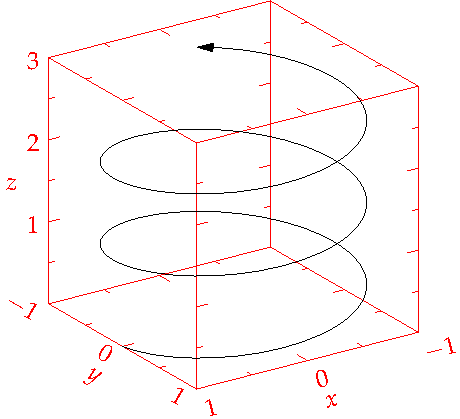
\includegraphics[width=\linewidth]{helix}
  \caption{This is a margin figure.  The helix is defined by 
    $x = \cos(2\pi z)$, $y = \sin(2\pi z)$, and $z = [0, 2.7]$.  The figure was
    drawn using Asymptote (\url{http://asymptote.sf.net/}).}
  \label{fig:marginfig}
\end{marginfigure}
\begin{Verbatim}
\begin{marginfigure}
  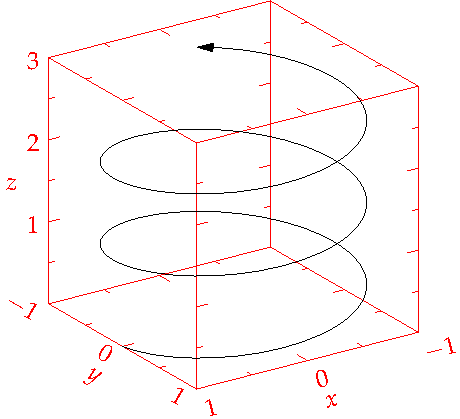
\includegraphics{helix}
  \caption{This is a margin figure.}
\end{marginfigure}
\end{Verbatim}

The \docenv{marginfigure} and \docenv{margintable} environments accept an optional parameter \docopt{offset} that adjusts the vertical position of the figure or table.  See the ``\nameref{sec:sidenotes}'' section above for examples.  The specifications are:
\begin{docspec}
  \doccmd{begin\{marginfigure\}[\docopt{offset}]}\\
  \qquad\ldots\\
  \doccmd{end\{marginfigure\}}\\
  \mbox{}\\
  \doccmd{begin\{margintable\}[\docopt{offset}]}\\
  \qquad\ldots\\
  \doccmd{end\{margintable\}}\\
\end{docspec}

Figure~\ref{fig:fullfig} is an example of the \Verb|figure*|
environment and figure~\ref{fig:textfig} is an example of the normal
\Verb|figure| environment.

\begin{figure*}[h]
  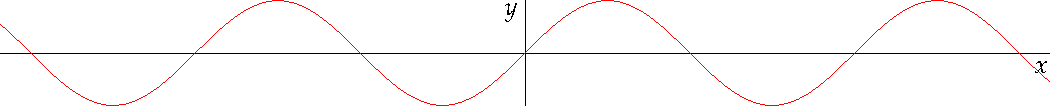
\includegraphics[width=\linewidth]{sine.pdf}%
  \caption{This graph shows $y = \sin x$ from about $x = [-10, 10]$.
  \emph{Notice that this figure takes up the full page width.}}%
  \label{fig:fullfig}%
\end{figure*}

\begin{figure}
  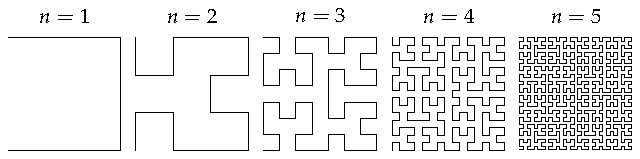
\includegraphics{hilbertcurves.pdf}
%  \checkparity This is an \pageparity\ page.%
  \caption{Hilbert curves of various degrees $n$.
  \emph{Notice that this figure only takes up the main textblock width.}}
  \label{fig:textfig}
  %\zsavepos{pos:textfig}
  \setfloatalignment{b}
\end{figure}

Table~\ref{tab:normaltab} shows table created with the \docpkg{booktabs}
package.  Notice the lack of vertical rules---they serve only to clutter
the table's data.

\begin{table}[ht]
  \centering
  \fontfamily{ppl}\selectfont
  \begin{tabular}{ll}
    \toprule
    Margin & Length \\
    \midrule
    Paper width & \unit[8\nicefrac{1}{2}]{inches} \\
    Paper height & \unit[11]{inches} \\
    Textblock width & \unit[6\nicefrac{1}{2}]{inches} \\
    Textblock/sidenote gutter & \unit[\nicefrac{3}{8}]{inches} \\
    Sidenote width & \unit[2]{inches} \\
    \bottomrule
  \end{tabular}
  \caption{Here are the dimensions of the various margins used in the Tufte-handout class.}
  \label{tab:normaltab}
  %\zsavepos{pos:normaltab}
\end{table}

\section{Full-width text blocks}

In addition to the new float types, there is a \docenv{fullwidth}
environment that stretches across the main text block and the sidenotes
area.

\begin{Verbatim}
\begin{fullwidth}
Lorem ipsum dolor sit amet...
\end{fullwidth}
\end{Verbatim}

\begin{fullwidth}
\small\itshape\lipsum[1]
\end{fullwidth}

\section{Typography}\label{sec:typography}

\subsection{Typefaces}\label{sec:typefaces}
If the Palatino, \textsf{Helvetica}, and \texttt{Bera Mono} typefaces are installed, this style
will use them automatically.  Otherwise, we'll fall back on the Computer Modern
typefaces.

\subsection{Letterspacing}\label{sec:letterspacing}
This document class includes two new commands and some improvements on
existing commands for letterspacing.

When setting strings of \allcaps{ALL CAPS} or \smallcaps{small caps}, the
letter\-spacing---that is, the spacing between the letters---should be
increased slightly.\cite{Bringhurst2005}  The \Verb|\allcaps| command has proper letterspacing for
strings of \allcaps{FULL CAPITAL LETTERS}, and the \Verb|\smallcaps| command
has letterspacing for \smallcaps{small capital letters}.  These commands
will also automatically convert the case of the text to upper- or
lowercase, respectively.

The \Verb|\textsc| command has also been redefined to include
letterspacing.  The case of the \Verb|\textsc| argument is left as is,
however.  This allows one to use both uppercase and lowercase letters:
\textsc{The Initial Letters Of The Words In This Sentence Are Capitalized.}



\section{Installation}\label{sec:installation}
To install the Tufte-\LaTeX\ classes, simply drop the
following files into the same directory as your \texttt{.tex}
file:
\begin{quote}
  \ttfamily
  tufte-common.def\\
  tufte-handout.cls\\
  tufte-book.cls
\end{quote}

% TODO add instructions for installing it globally



\section{More Documentation}\label{sec:more-doc}
For more documentation on the Tufte-\LaTeX{} document classes (including commands not
mentioned in this handout), please see the sample book.

\section{Support}\label{sec:support}

The website for the Tufte-\LaTeX\ packages is located at
\url{http://code.google.com/p/tufte-latex/}.  On our website, you'll find
links to our \smallcaps{svn} repository, mailing lists, bug tracker, and documentation.

\bibliography{sample-handout}
\bibliographystyle{plainnat}



\end{document}